\documentclass[default]{beamer}
\setbeamertemplate{navigation symbols}{}
\setbeamertemplate{theorems}[numbered]
\usetheme{CambridgeUS}
\useoutertheme{infolines}
%\usecolortheme{crane}

\usepackage{cmap}	% Поддержка поиска русских слов в PDF (pdflatex)
\usepackage[T2A]{fontenc}       %поддержка кириллицы
\usepackage[utf8]{inputenc}	% Выбор языка и кодировки
\usepackage[english, russian]{babel}
%\usepackage[unicode]{hyperref}			% Русский язык для оглавления pdf
%\usepackage{bookmark}					% Оглавление в pdf
\usepackage{caption}
\usepackage{xcolor}

\graphicspath{{../../images/ai/}} 			% Пути к изображениям

\let\Theorem\relax
\newtheorem{Theorem}{Теорема}
\newtheorem{Pred}{Утверждение}
\newtheorem{Def}{Определение}

\makeatletter
\setbeamertemplate{footline}
{
	\leavevmode%
	\hbox{%
		\begin{beamercolorbox}[wd=.333333\paperwidth,ht=2.25ex,dp=1ex,center]{author
				in head/foot}%
			\usebeamerfont{author in
				head/foot}\insertshortauthor~~\beamer@ifempty{\insertshortinstitute}{}{(\insertshortinstitute)}
		\end{beamercolorbox}%
		\begin{beamercolorbox}[wd=.333333\paperwidth,ht=2.25ex,dp=1ex,center]{title in
				head/foot}%
			\usebeamerfont{title in head/foot}\insertshorttitle
		\end{beamercolorbox}%
		\begin{beamercolorbox}[wd=.333333\paperwidth,ht=2.25ex,dp=1ex,right]{date in
				head/foot}%
			\usebeamerfont{date in head/foot}\insertshortdate{}\hspace*{2em}
			\insertframenumber{}\hspace*{2ex} 
		\end{beamercolorbox}
	}%
	\vskip0pt%
}

\begin{document}
	
	\title[Введение в ИИ. ДИС]{Введение в искусственный интеллект.\\Динамические интеллектуальные системы}
	\author[Панов]{Александр Панов}
	\institute[ИСА~РАН]{Интситут системного анализа РАН}
	\date{02 марта 2015 г.} 
	
	\begin{frame}
		\titlepage
	\end{frame}
	
	\section {Динамические системы, основанные не правилах}
	\subsection{Введение}
	\begin{frame}
		\frametitle{Истоки проблемы}
		\begin{itemize}
			\item Сложность задач управления.
			\item Существенная роль экспертных суждений и знаний человека.
			\item Применение подходов, в которых в качестве значений переменных допускаются не только числа, но и слова или предложения искусственного или естественного языка.
		\end{itemize}
	\end{frame}

	\begin{frame}
		\frametitle{Пример области применения}
		
		Двухуровневые системы управления в беспилотных автономных вертолётах и квадракоптерах.
		\begin{itemize}
			\item \textbf{Стратегический} (или, как иногда говорят, делиберативный) уровень управления, решающий задачи, например, планирования полёта или выбора траектории или выбора цели.
			\item \textbf{Реактивный} уровень управления реализует требуемые действия. 
		\end{itemize}
	\end{frame}

	\begin{frame}
		\frametitle{Пример модельной задачи}
		
		Задача управления движением автомобилей на нерегулируемом перекрёстке.
		\begin{itemize}
			\item Решения о действии в соответствии с правилами дорожного движения принимаются на делиберативном уровне с помощью применения систем правил.
			\item На реактивном уровне применяются соответствующие модели обгона или левого поворота.
		\end{itemize}
		\par\bigskip
		\begin{figure}
			\centering
			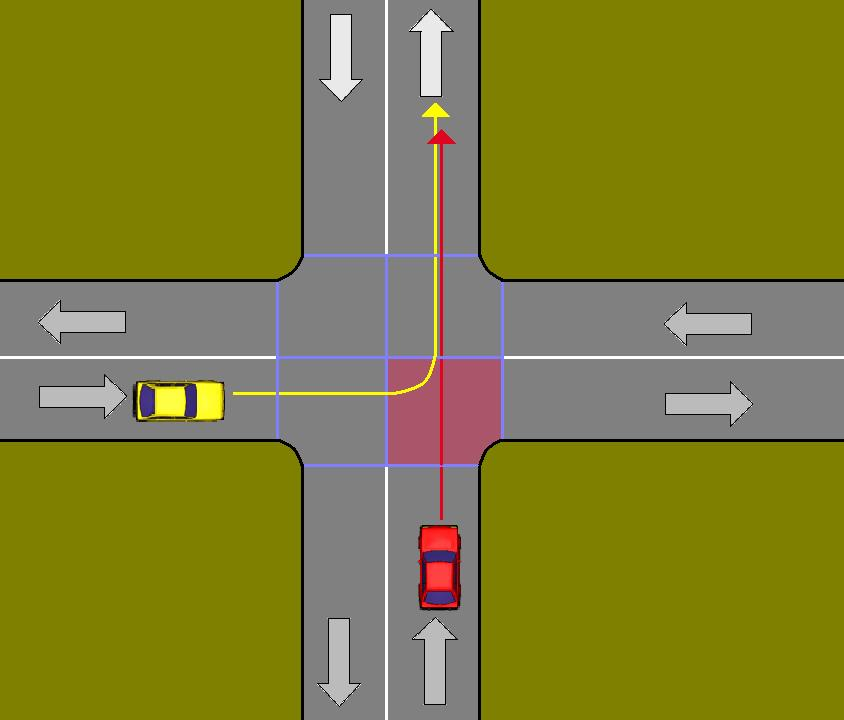
\includegraphics[width=0.35\textwidth]{dyn_cars.jpg}
		\end{figure}
	\end{frame}
					
	\subsection{Постановка задачи}

	\begin{frame}
		\frametitle{Правила}
		
		Правилом называется упорядоченная тройка множеств $r=<C,A,D>$, где
		\begin{itemize}
			\item $C$ "--- условие правила,
			\item $A$ "--- множество добавляемых правилом фактов,
			\item $D$ "--- множество удаляемых правилом фактов.
		\end{itemize}
		\par\bigskip
		Выделим в формулах из указанных множеств сорт переменной $t$, соответствующей дискретному времени: $t\in T$, где $T$ "--- дискретное упорядоченное множество.
		
		\begin{Def}
			Будем говорить, что условие правила выполнено, если в $n$-ом состоянии рабочей памяти истинна каждая из атомарных формул условия, в которой $t=n$, где $n\in T$.
		\end{Def}
	\end{frame}

	\begin{frame}
		\frametitle{Цели курса}
		
		Множество правил $\Pi$ разбивается на два подмножества:
		\begin{itemize}
			\item подмножество правил $\Pi_{CL}$, не соответствующих никаким действиям, а лишь пополняющих множество фактов состояния "--- \textbf{правила  замыкания}, значения переменной $t$ одни и те же в формулах условия и в формулах из множеств добавляемых и удаляемых фактов;
			\item подмножество правил $\Pi_{TR}$, являющихся, по существу, некоторыми действиями и, поэтому изменяющих состояние системы "--- \textbf{правила переходов}, в формулах из множеств удаляемых и добавляемых фактов этих правил значения переменной $t$, по крайней мере, на единицу больше, чем в формулах условия.
		\end{itemize}

		\begin{equation}
			\Pi_{CL}= <C(t),A(t),D(t)>, \Pi_{TR} = <C(t),A(t+1),D(t+1)>.
		\end{equation}
	\end{frame}

	\begin{frame}
		\frametitle{Стратегия $CL$ применения правил}

		Стратегия $CL$:
		\begin{enumerate}
			\item Выбрать некоторое правило $r$ из множества правил $\Pi_{CL}$.
			\item Проверить выполнимость условия $С$ правила $r$ в текущем состоянии рабочей памяти.
			\item Если $С$ выполнено, то подставить на места всех свободных переменных в формулы правила соответствующие значения из рабочей памяти. Иначе перейти к п.1.
			\item  Применить правило, т.~е. записать в текущее состояние рабочей памяти те значения, на которых оказались выполненными формулы из $А$ и удалить из рабочей памяти значения, на которых оказались выполнены формулы из $D$.  
			\item Перейти к п.1.
		\end{enumerate}

		Работа стратегии завершается со стабилизацией текущего состояния рабочей памяти. По наступлении стабилизации начинает выполняться стратегия $TR$.		
	\end{frame}

	\begin{frame}
		\frametitle{Стратегия $TR$ применения правил}
		
		Стратегия $TR$:
		\begin{enumerate}
			\item Выбрать некоторое правило $r$ из множества правил $\Pi_{TR}$.
			\item Проверить выполнимость условия $С$ правила $r$ в текущем состоянии рабочей памяти.
			\item Если $С$ выполнено, то подставить на места всех свободных переменных в формулы правила соответствующие значения из рабочей памяти. Иначе перейти к п.1.
			\item  Применить правило, т.~е. записать в текущее состояние рабочей памяти те значения, на которых оказались выполненными формулы из $А$ и удалить из рабочей памяти значения, на которых оказались выполнены формулы из $D$.  
			\item Перейти к стратегии $CL$.
		\end{enumerate}
		
	\end{frame}

	\begin{frame}
		\frametitle{ДИС, основанная на правилах}
		
		Пусть $Х$ "--- множество фактов. 
		\begin{itemize}
			\item каждое правило из $\Pi_{CL}$ можно рассматривать как некоторое отображение из $2^X$ в $2^X$,
			\item каждое правило из $\Pi_{TR}$ "--- как некоторое отображение из $2^X\times T$ в $2^X$.
		\end{itemize}
		\par\bigskip
		Если $\chi(t) = \chi\in 2^X$, то
		\begin{itemize}
			 \item $(CL,\chi)=\Phi(\chi)$ "--- функция замыкания,
			 \item $(TR,\chi)=\Psi(\chi,t)$ "--- функция переходов.
		\end{itemize}
		\par\bigskip
		\begin{Def}
			Четвёрку  
			\begin{equation}
				D=<X,T,\Phi,\Psi>,
			\end{equation}
			где $\Phi:2^X\rightarrow 2^X$, $\Psi:2^X\times T\rightarrow 2^X$,будем называть динамической системой, основанной на правилах.
		\end{Def}
	\end{frame}
	
	\begin{frame}
		\frametitle{Состояния ДИС и её траектория}
		
		Роль стратегии $CL$ и функции $\Phi$ системы $D$ заключаются в пополнении описания текущего состояния. Этот процесс завершается при стабилизации состояния:
		\begin{equation}\label{eq:stabil}
			\Phi(\chi)=\chi.
		\end{equation}
		\begin{Def}
			Траекторией системы  D называется множество
			\begin{equation}
				\Xi=\{\Phi(\Psi(\chi(t),t))|t\in T\},
			\end{equation}
			где $\chi(t)$ "--- решение уравнения (\ref{eq:stabil}).
		\end{Def}
		
		Иначе уравнение траектории системы $D$ можно записать следующим образом:
		\begin{equation}
			\chi(t+1)=\Phi(\Psi(\chi(t),t)).
		\end{equation}
	\end{frame}

	\subsection{Управляемые ДИС}

	\begin{frame}
		\frametitle{Управляемые ДИС, основанные на правилах}
		
		\begin{Def}
			Система
			\begin{equation}\label{def:cdis}
				K=<X,T,\Phi,\Psi,U>,
			\end{equation}
			где $X$, $T$, $\Phi$ и $\Psi$ были определены выше, а $U: 2^X\times T \rightarrow 2^X$, называется управляемой динамической системой, основанной на правилах. 
		\end{Def}
		
		Функция $U$ реализуется стратегией применения правил управления $CN$ и множеством правил управления $\Pi_{CN}$.
		
		Траектория системы (\ref{def:cdis}) запишется в следующем виде:
		\begin{equation}\label{eq:control}
			\chi(t+1)=\Phi(\Psi(\chi(t),t)\cup U(\chi(t),t)).
		\end{equation}
	\end{frame}

	\begin{frame}
		\frametitle{Возмущения}
		
		\begin{Def}
			Под возмущением понимается некоторое множество событий $\delta(t)$, появление которого в состоянии $\chi(t)$ не является результатом решения уравнений \ref{eq:stabil}.
		\end{Def}
		Если $\delta(t)\in 2^X $, тогда, в отсутствие управления
		\begin{equation}
			\chi(t+1) =\Phi(\Psi(\underbrace{\Phi(\chi(t)\cup\delta(t))}_{\chi'(t)},t)).
		\end{equation}
		\begin{Def}
			Траектория $\Xi$ называется устойчивой, если для любого $t$ и возмущения $\delta(t)$ 
			\begin{equation}
				\Phi(\Psi(\chi(t),t))\subseteq\Phi(\Psi(\underbrace{\Phi(\chi(t)\cup\delta(t))}_{\chi'(t)},t)).
			\end{equation}
		\end{Def}
		
	\end{frame}

	\begin{frame}
		\frametitle{Достаточное условие устойчивости}
		
		Пусть $\chi_1,\chi_2\in 2^X$.
		\begin{Def}
			Функцию $\Phi$ будем называть монотонной, если из $\chi_1\subseteq\chi_2$ следует $\Phi(\chi_1)\subseteq\Phi(\chi2)$.
		\end{Def}
		
		\begin{Def}
			Функцию $\Psi$ будем называть монотонной по переменной состояния, если из $\chi_1\subseteq\chi_2$ следует $\Psi(\chi_1,\cdot)\subseteq\Psi(\chi_2,\cdot)$.
		\end{Def}
		
		\begin{Pred}[достаточное условие устойчивости]
			Траектория $\Xi$ системы (\ref{eq:vosm}) устойчива, если функция $\Phi$ монотонна, а $\Psi$ монотонна по переменной состояния.
			
		\end{Pred}		
	\end{frame}

	\begin{frame}
		\frametitle{Управление и возмущения}
		
		Рассмотрим теперь более общий случай, когда возмущение присутствует в управляемой системе, т.~е рассмотрим систему
		\begin{equation}\label{eq:contr_vosm}
			\chi(t+1) =\Phi(\underbrace{\Psi(\Phi(\chi(t)\cup\delta(t)),t)}_{\chi'(t+1)}\cup U(\chi'(t+1),t+1)).
		\end{equation}
		Вопрос: каким образом, располагая управлением $U$, компенсировать влияние возмущения $\delta$ на поведение системы (\ref{eq:contr_vosm}), если её траектория неустойчива?
		\par\bigskip
		В силу непрогнозируемости среды, появление возмущения $\delta(t)$ в состоянии $\chi(t)$ предвидеть невозможно, поэтому применение управления $U$ для компенсации этого возмущения  возможно не ранее следующего состояния, т.~е.  состояния 
		\begin{equation}
			\chi(t+1)=\Phi(\Psi(\Phi(\chi(t)\cup\delta(t)),t)).
		\end{equation}
	\end{frame}

	\begin{frame}
		\frametitle{Компенсация возмущения}
		
		\begin{Theorem}\label{th:compens}
			Для компенсации возмущения $\delta(t)$ системы (\ref{eq:contr_vosm}) достаточно применения управления:
			\begin{eqnarray}
				U(\chi'(t+1),t+1)=\Phi(\Psi(\chi(t+1),t+1))\setminus\nonumber\\
				\Phi(\Psi(\underbrace{\Phi(\Psi(\Phi(\chi(t)\cup\delta(t)),t))}_{\chi'(t+1)},t+1)).
			\end{eqnarray}
		\end{Theorem}
	\end{frame}

	\subsection{Синтез управления}

	\begin{frame}
		\frametitle{Задача компенсации возмущений}
		
		В динамических системах, основанных на правилах, множество допустимых управлений определяется множеством $\Pi_{CN}$ "--- правил управления. 
		\par\bigskip
		Задача компенсации возмущения, с этой точки зрения состоит в подборе таких правил из множества  $\Pi_{CN}$, которые обеспечивают требуемую коррекцию поведения системы, т.~е. возврат очередного состояния на расчётную траекторию.
	\end{frame}

	\begin{frame}
		\frametitle{Ранги}
		
		\begin{Def}
			Если $r=<C,A,D>$ "--- некоторое правило, то величина $rank(r) = |A|-|D|$, (где $|A|$ и $|D|$ "--- мощности соответствующих множеств), называется рангом правила $r$. 
		\end{Def}
		
		\begin{Def}
			Последовательность правил, доставляющих решение уравнению (\ref{eq:stabil}): $\Phi(\chi)=\chi$ называется полной последовательностью.
		\end{Def}
		\par\bigskip
		Для простоты будем считать, что для всех правил множества добавляемых фактов попарно не пересекаются.
	\end{frame}

	\begin{frame}
		\frametitle{Монотонность и полнота}
		
		\begin{Pred}
			Функция $\Phi$ монотонна тогда и только тогда, когда для всякой полной последовательности из $N$ попарно применимых правил в множестве правил $\Pi_{CL}$ выполняется
			\begin{equation}
				\sum_{i=1}^{N}rank(r_i)\geqslant N.
			\end{equation}
		\end{Pred}
		
		\begin{Pred}
			Функция $\Psi$ монотонна тогда и только тогда, когда для каждого правила $r$ в множестве $\Pi_{TR}$ $rank(r)\geqslant 1$.
		\end{Pred}
	\end{frame}

	\begin{frame}
		\frametitle{Задача синтеза управления}
		
		Теорема (\ref{th:compens}) говорит о принципиальной возможности существования такого управления, которое может компенсировать любое возмущение системы (\ref{eq:contr_vosm}).
		
		Вопрос: как построить такое управление?
		
		\begin{Def}
			Рангом факта $F$ в последовательности правил $\Pi$ называется величина
			\begin{equation}
				rank_{\Pi}(F)=rank_{\Pi}(F_F)-rank_{\Pi}(F_D),
			\end{equation}
			где $rank_{\Pi}(F_A)$ "--- количество вхождений факта $F$ в множества добавляемых фактов правил из $\Pi$, а $rank_{\Pi}(F_D)$ "--- количество вхождений факта $F$ в множества удаляемых фактов правил из $\Pi$ (при этом вычитание производится только из предшествующего правила последовательности $\Pi$, содержащего $F$ в списке добавлений).
		\end{Def}
	\end{frame}

	\begin{frame}
		\frametitle{Стратегия $CN$}
		
		\begin{enumerate}
			\item Выбрать очередной факт $F_i$ из множества  $\Delta_0 = \Phi(\Psi(\chi(t+1)),t+1))\setminus \Phi(\Psi(\chi'(t+1)),t+1))$.
			\item Выбрать из множества $\Pi_{CN}$ такое правило $r$, что $F_i\in A(r)$ и $rank_{\Pi}(F_i)\geqslant 1$. Если $C(r)\subset\chi'(t+1)$ "--- работа стратегии завершена.
			\item Построить множество $\Delta_{j+1} = \Delta_j \cup C(r)\cup D(r)\setminus A(r)$.
			\item Выбрать из множества $\Pi_{CN}$ такое правило $r$, что $A(r)\cap\Delta_{j+1}\not=\varnothing$ и $rank_{\Pi}(F_i)\geqslant 1$. Если $C(r)\subseteq\chi'(t+1)$ "--- работа стратегии для факта $F_i$ завершена.
			\item Если множество $\Delta_0$ исчерпано, то работа стратегии полностью завершена, иначе $i := i+1$ и переход к шагу 1.
		\end{enumerate}
	\end{frame}	

	\begin{frame}
		\frametitle{Существование управления}
		
		\begin{Theorem}
			Управление $U(\chi'(t+1),t+1))$ системы (\ref*{eq:contr_vosm}) существует тогда и только тогда, когда для каждого факта
			\[ F_i\in\Phi(\Psi(\chi(t+1)),t+1))\setminus\Phi(\Psi(\Phi(\Psi(\Phi(\chi(t)\cup\delta(t)),t)), t+1))
			\]
			найдётся последовательность $\Pi$ попарно применимых правил в множестве $\Pi_{CN}$, такая что 
			\[
			C(r_1)\subseteq\Phi(\Psi(\Phi(\Psi(\Phi(\chi(t)\cup\delta(t)),t))
			\] 
			и $rank_{\Pi}(F_i)\geqslant 1$, где $С(r_1)$ условие первого правила последовательности $\Pi$.
		\end{Theorem}
	\end{frame}

	\subsection{Обратная связь}

	\begin{frame}
		\frametitle{Замыкание уонтура управления}
		
		Если замкнуть контур управления, то устойчивость системы можно повысить включением в контур управления механизма обратной связи.
		\par\bigskip
		Методы синтеза обратной связи позволяют компенсировать возмущение в том состоянии, в котором наблюдается эффект последнего.
		
		\begin{Theorem}
			Для компенсации возмущения $\delta(t)$ системы (\ref{eq:contr_vosm})  в состоянии $\chi(t+1)$ достаточно применения обратной связи:
			\begin{equation}
				\Omega(\chi(t+1)) = \chi(t+1) \setminus \Phi(\Psi(\Phi(\chi(t)\cup\delta(t)),t)).
			\end{equation}
		\end{Theorem}
	\end{frame}
	
	\begin{frame}
		\frametitle{Стратегия $CB$}
		
		\begin{enumerate}
			\item Выбрать очередной факт $F_i$ из множества  $\Delta_0 = \chi(t+1)\setminus\chi'(t+1)$.
			\item Выбрать из множества $\Pi_{CB}$ такое правило $r$, что $F_i\in A(r)$ и $rank_{\Pi}(F_i)\geqslant 1$. Если $C(r)\subset\chi'(t+1)$ "--- работа стратегии завершена.
			\item Построить множество $\Delta_{j+1} = \Delta_j \cup C(r)\cup D(r)\setminus A(r)$.
			\item Выбрать из множества $\Pi_{CB}$ такое правило $r$, что $A(r)\cap\Delta_{j+1}\not=\varnothing$ и $rank_{\Pi}(F_i)\geqslant 1$. Если $С(r)\subseteq\chi'(t+1)$ "--- работа стратегии для факта $F_i$ завершена.
			\item Если множество $\Delta_0$ исчерпано, то работа стратегии полностью завершена, иначе $i := i+1$ и переход к шагу 1.
		\end{enumerate}
	\end{frame}	
		
	\begin{frame}
		\frametitle{Задача управляемости системы}
		
		Будем рассматривать системы (\ref{eq:control})
		\[
		\chi(t+1)=\Phi(\Psi(\chi(t),t)\cup U(\chi(t),t)).
		\]
		\par\bigskip
		Если задана пара точек $(\chi_0, \chi_1)\in 2^X\times 2^X$, то задача управляемости системы (\ref*{eq:control}) состоит в установлении условий существования значений управления $U(\chi(t),t)$, позволяющих перевести систему (\ref*{eq:control}) из состояния $\chi(0)\subseteq\chi_0$ в состояние $\chi(N)$, такое что $\chi_1\subseteq\chi(N)$, где $N\in T$.
	\end{frame}

		
	\begin{frame}
		\frametitle{Достижимость состояний}
		
		\begin{Def}
			Если $2^X$ "--- множество состояний системы (\ref{eq:control}), то пара точек $(\chi_0, \chi_1)$ в $2^X\times 2^X$  называется $N$-достижимой, если  существуют такие значения управления $U(\chi(t),t)$ ($t=0,1,\dots,N-1$) системы (\ref{eq:control}) , что $\chi_1\times\chi(N)$, при начальных условиях $\chi(0)\subseteq\chi_0$, где $\chi(N)$ "--- решение уравнения (\ref{eq:control}).
		\end{Def}
		\begin{Def}
			Система (\ref{eq:control}) называется вполне достижимой если для любой пары точек  $(\chi_0, \chi_1)\in 2^X\times 2^X$  существует $N\in T$, такое что пара $(\chi_0, \chi_1)$ является $N$-достижимой.
		\end{Def}
	\end{frame}

	\begin{frame}
		\frametitle{Управляемость системы}
		
		\begin{Theorem}
			Пара точек $(\chi_0, \chi_1)$ системы (\ref{eq:control})  $N$-достижима тогда и только тогда когда для каждого факта $F_i\in\chi_1$ в множестве $\Pi_{CN}$ найдётся последовательность $\Pi$ попарно применимых правил, такая что $C(r_1)\subseteq\chi_0$ и $rank_{\Pi}(F_i)\geqslant 1$, где $C(r_1)$ условие первого правила последовательности $\Pi$.
		\end{Theorem}
		
		\begin{Theorem}
			Система (\ref*{eq:control})  вполне достижима если и только если: 
			\begin{enumerate}
				\item для всякого $F_i\in X$ $F_i\in A$, где $A$ "--- множество добавляемых фактов одного из правил,
				\item существует последовательность $\Pi$, состоящая из всех правил $\Pi_{CN}$, что для всякого $F$ из $\Pi_{CN}$ $rank_{\Pi}(F)\geqslant 1$.
			\end{enumerate}
		\end{Theorem}
	\end{frame}
			
	%	\begin{frame}
	%		\frametitle{Цели курса}
	%		
	%		\begin{itemize}
	%			\item
	%		\end{itemize}
	%	\end{frame}
	
\end{document}
	
	
